\section{Pendahuluan}
\subsection{Latar Belakang}
Praktikum ini dilakukan untuk mempelajari topologi jaringan dan mempersiapkan mahasiswa agar dapat melakukan crimping dan routing IPv4 pada perangkat elektronik pintar.

\subsubsection{Dasar Teori}

Jaringan komputer adalah kumpulan perangkat seperti komputer, printer, dan perangkat lainnya yang saling terhubung untuk berbagi sumber daya dan informasi. Konsep dasar jaringan mirip dengan hubungan antar rumah dalam suatu kompleks: rumah sebagai komputer, jalan sebagai kabel jaringan, dan tukang pos sebagai router.

Jaringan memungkinkan transfer data secara cepat dan efisien tanpa perlu alat tambahan seperti USB. Keberadaan jaringan tidak hanya membuat proses komunikasi antar perangkat menjadi lebih praktis, tetapi juga mendukung efisiensi operasional, produktivitas, dan fleksibilitas dalam berbagai lingkungan seperti rumah, kantor, dan institusi pendidikan.

\\{Jenis-Jenis Jaringan}
Jaringan komputer dapat diklasifikasikan berdasarkan cakupan geografisnya:
\begin{itemize}
    \item \textbf{Personal Area Network (PAN)}: Jaringan kecil yang digunakan untuk perangkat pribadi seperti smartphone, laptop, dan printer.
    \item \textbf{Local Area Network (LAN)}: Menghubungkan perangkat dalam area terbatas, seperti dalam satu gedung. Biasanya digunakan di kantor atau laboratorium.
    \item \textbf{Campus Area Network (CAN)}: Digunakan untuk menghubungkan beberapa LAN dalam area kampus atau kompleks gedung.
    \item \textbf{Metropolitan Area Network (MAN)}: Menghubungkan jaringan dalam satu kota atau wilayah yang lebih luas dari CAN.
    \item \textbf{Wide Area Network (WAN)}: Jaringan berskala global yang menghubungkan berbagai jaringan di berbagai lokasi geografis, contohnya adalah internet.
\end{itemize}


Dalam jaringan komputer, \textbf{protokol} adalah seperangkat aturan yang mengatur komunikasi antar perangkat. Tanpa protokol, perangkat yang terhubung tidak dapat saling memahami dan bertukar data dengan benar.

\\{Jenis Protokol}
Terdapat tiga kategori utama protokol dalam jaringan komputer:
\begin{enumerate}
    \item \textbf{Protokol Komunikasi}, seperti:
    \begin{itemize}
        \item \textbf{HTTP/HTTPS}: Digunakan untuk mengakses dan mengamankan komunikasi web.
        \item \textbf{FTP}: Untuk transfer file antar perangkat.
        \item \textbf{TCP/IP}: Mengatur pengalamatan dan pengiriman data secara andal.
    \end{itemize}
    \item \textbf{Protokol Keamanan}: Menjamin data tidak disadap atau diubah selama transmisi, seperti SSL/TLS.
    \item \textbf{Protokol Manajemen}: Seperti DHCP, yang mengatur pemberian alamat IP secara otomatis kepada perangkat dalam jaringan.
\end{enumerate}

\\{IP Address dan Subnetting}
Setiap perangkat dalam jaringan memiliki \textbf{alamat IP (Internet Protocol Address)} yang berfungsi sebagai identitas unik. Alamat ini terbagi menjadi:
\begin{itemize}
    \item \textbf{Private IP Address}: Digunakan dalam jaringan lokal dan tidak bisa diakses langsung dari internet.
    \item \textbf{Public IP Address}: Diberikan oleh ISP dan digunakan untuk berkomunikasi dengan internet.
\end{itemize}

IP Address juga dapat diklasifikasikan sebagai \textbf{statis} (tetap) atau \textbf{dinamis} (berubah-ubah). Untuk efisiensi dan pengelolaan jaringan, IP address dapat dibagi menggunakan teknik \textbf{subnetting} dengan bantuan \textbf{subnet mask} dan \textbf{prefix (CIDR)}. Hal ini memungkinkan pembagian jaringan besar menjadi beberapa jaringan kecil (subnet) yang lebih mudah dikelola.


%===========================================================%
\section{Tugas Pendahuluan}
\begin{enumerate}
    \item \textbf{Alokasi IP Address dan Prefix Subnet (CIDR):}
    
    Diberikan 4 departemen dengan jumlah perangkat berbeda, maka subnet yang dibutuhkan adalah:
    
    \begin{itemize}
        \item \textbf{Departemen Produksi (50 perangkat)}: butuh minimal 64 IP $\Rightarrow$ gunakan prefix /26 \\
        \textbf{Network}: 192.168.1.0/26 \\
        \textbf{Range Host}: 192.168.1.1 – 192.168.1.62 \\
        \textbf{Broadcast}: 192.168.1.63
        \item \textbf{Departemen Administrasi (20 perangkat)}: butuh minimal 32 IP $\Rightarrow$ gunakan prefix /27 \\
        \textbf{Network}: 192.168.1.64/27 \\
        \textbf{Range Host}: 192.168.1.65 – 192.168.1.94 \\
        \textbf{Broadcast}: 192.168.1.95
        \item \textbf{Departemen Keuangan (10 perangkat)}: butuh minimal 16 IP $\Rightarrow$ gunakan prefix /28 \\
        \textbf{Network}: 192.168.1.96/28 \\
        \textbf{Range Host}: 192.168.1.97 – 192.168.1.110 \\
        \textbf{Broadcast}: 192.168.1.111
        \item \textbf{Departemen R\&D (100 perangkat)}: butuh minimal 128 IP $\Rightarrow$ gunakan prefix /25 \\
        \textbf{Network}: 192.168.1.112/25 \\
        \textbf{Range Host}: 192.168.1.113 – 192.168.1.254 \\
        \textbf{Broadcast}: 192.168.1.255
    \end{itemize}
    
    \item \textbf{Topologi Sederhana Jaringan:}
    
    Semua subnet dihubungkan melalui satu \textbf{router utama}. Berikut gambar topologinya:
    
   \begin{figure}[H]
  \centering
  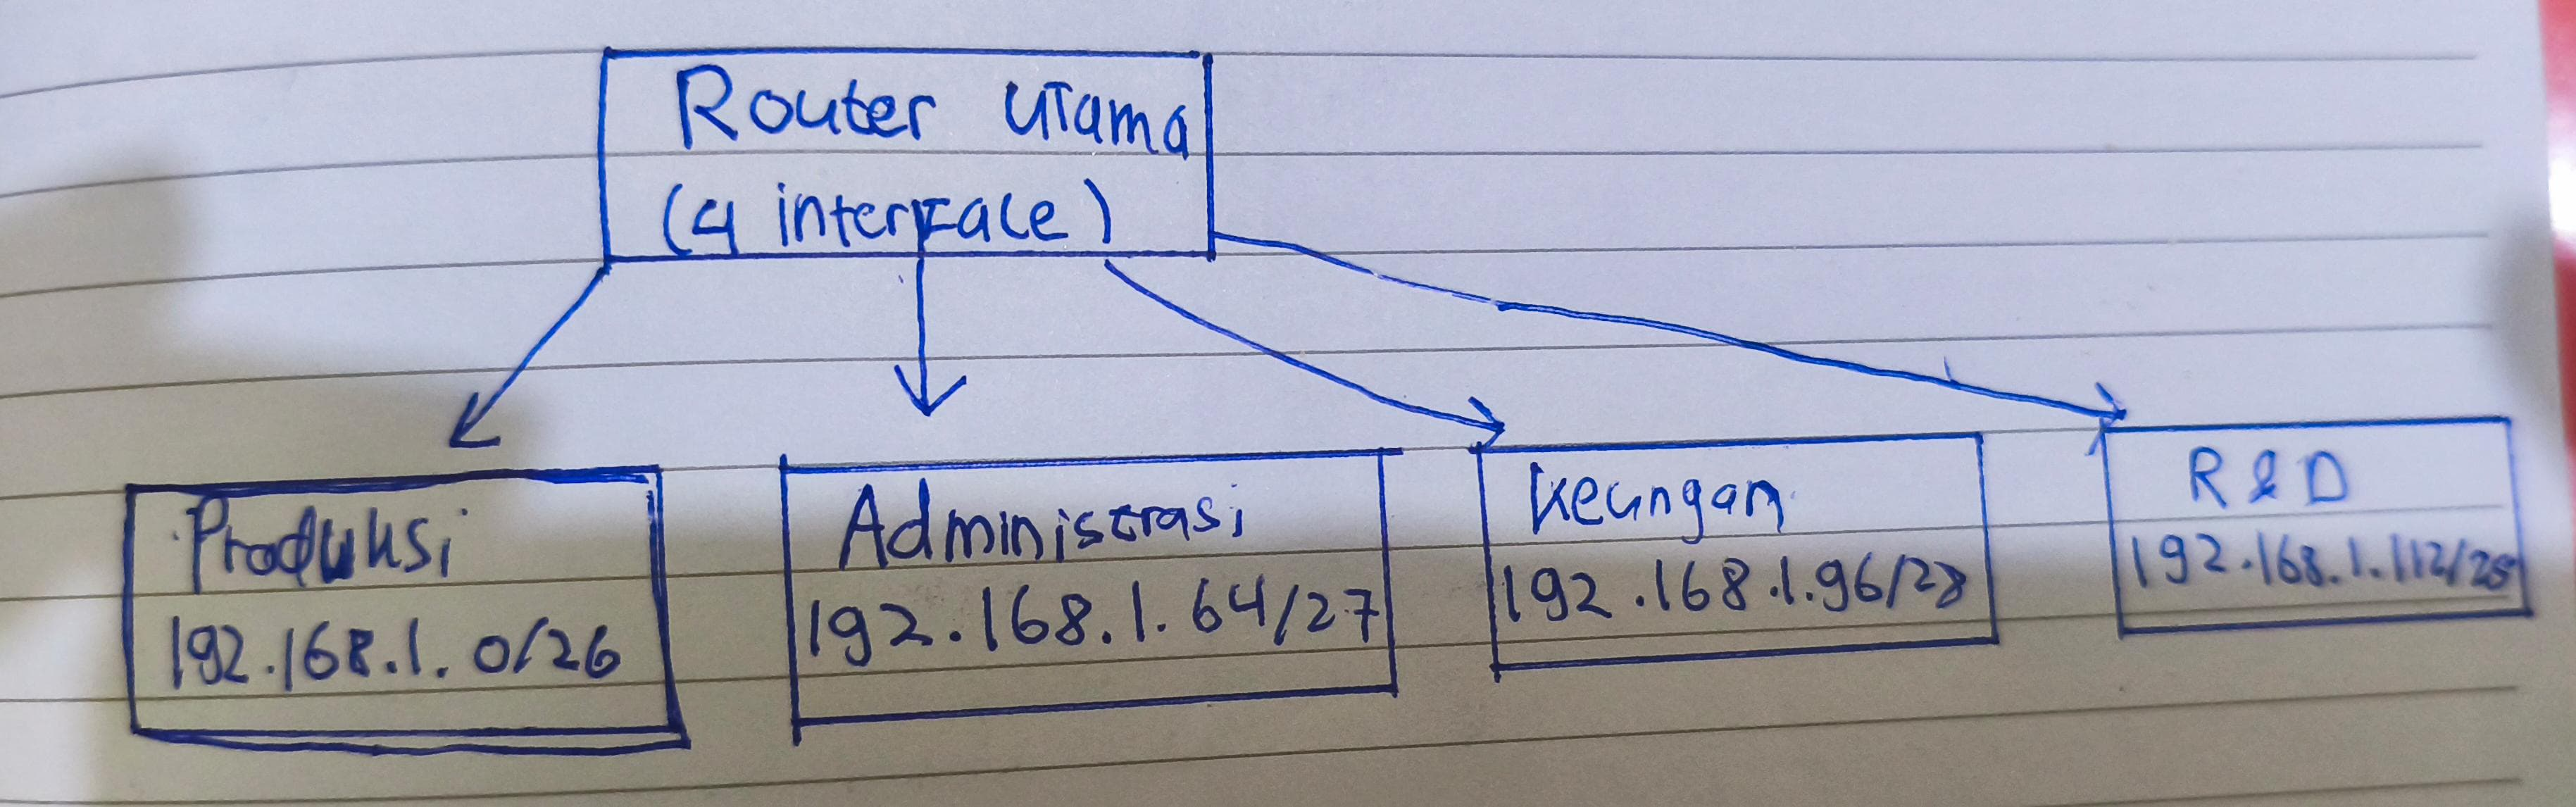
\includegraphics[width=1\linewidth]{P1/img/1.jpeg}
  \caption{Hasil pembuatan wiring schematic} 
  \label{fig:inirujukan}
\end{figure}


    \item \textbf{Tabel Routing Sederhana:}

    \begin{center}
    \begin{tabular}{|l|l|l|l|}
    \hline
    \textbf{Network Destination} & \textbf{Prefix} & \textbf{Gateway} & \textbf{Interface} \\
    \hline
    192.168.1.0      & /26  & - (direct) & eth0 \\
    192.168.1.64     & /27  & - (direct) & eth1 \\
    192.168.1.96     & /28  & - (direct) & eth2 \\
    192.168.1.112    & /25  & - (direct) & eth3 \\
    \hline
    \end{tabular}
    \end{center}

    \item \textbf{Jenis Routing yang Paling Cocok:}

    Routing yang paling cocok untuk jaringan ini adalah \textbf{Static Routing}, karena:
    \begin{itemize}
        \item Jumlah subnet tidak banyak (hanya 4 subnet).
        \item Topologi tidak kompleks dan jarang berubah.
        \item Konfigurasi lebih sederhana dan tidak membutuhkan overhead pertukaran informasi routing.
    \end{itemize}

    Jika ke depannya jaringan berkembang, maka dapat mempertimbangkan \textbf{Dynamic Routing} seperti OSPF untuk efisiensi dalam manajemen rute.
\end{enumerate}
